\documentclass[12pt]{article}
% ============================================================================
% PACKAGE IMPORTS — FINAL, PUBLICATION-READY
% ============================================================================
% --- Geometry (load early) ---
\usepackage[margin=1in]{geometry}
\setlength{\headheight}{14pt}

% --- Math & Symbols ---
\usepackage{amsmath,amssymb}
\usepackage{siunitx}

% --- Tables ---
\usepackage{array}
\usepackage{booktabs}
\usepackage{multirow}

% --- Graphics & Figures ---
\usepackage{graphicx}
\usepackage{float}
\usepackage{caption}
\usepackage{subcaption}

% --- TikZ & PGFPlots ---
\usepackage{tikz}
\usetikzlibrary{shapes.geometric, arrows.meta, positioning, shadows, fit, calc, decorations.pathmorphing, shapes.symbols}
\usepackage{pgfplots}
\pgfplotsset{compat=1.18}

% --- Lists ---
\usepackage{enumitem}

% --- Colors & Boxes ---
\usepackage{xcolor}
\usepackage[framemethod=TikZ]{mdframed}

% --- Typography & Spacing ---
\usepackage{setspace}
\usepackage{lineno}

% --- Headers & Footers ---
\usepackage{fancyhdr}

% --- Bibliography ---
\usepackage[numbers,sort&compress]{natbib}

% --- Hyperlinks (load near end) ---
\usepackage[hidelinks]{hyperref}

% ============================================================================
% SIUNITX CONFIGURATION — FINAL, PUBLICATION-READY
% ============================================================================
\sisetup{
    range-phrase = --,
    range-units = single,
    detect-all,
    separate-uncertainty = true
}

% ============================================================================
% PAGE LAYOUT — FINAL, PUBLICATION-READY
% ============================================================================
\onehalfspacing
\setlength{\parindent}{15pt}
\setlength{\parskip}{6pt}

\pagestyle{fancy}
\fancyhf{}
\rhead{\small Hybrid mRNA Vaccine for Glioblastoma}
\rfoot{\thepage}
\renewcommand{\headrulewidth}{0.5pt}

% ============================================================================
% HYPERREF SETUP — FINAL, PUBLICATION-READY
% ============================================================================
\hypersetup{
    colorlinks=true,
    linkcolor=black,
    urlcolor=blue,
    citecolor=black,
    pdfauthor={Collin B. George},
    pdftitle={Hybrid mRNA Vaccine for Glioblastoma},
    pdfkeywords={glioblastoma, mRNA vaccine, blood-brain barrier, neoantigens, focused ultrasound, immunotherapy, IL-12, RIG-I ligands}
}

% ============================================================================
% TITLE AND AUTHOR INFORMATION — FINAL, PUBLICATION-READY
% ============================================================================
\title{\textbf{A Translational Framework for a Hybrid mRNA Vaccine Targeting Glioblastoma:\\
Integrating Innate Priming, Personalized Neoantigens, and Blood--Brain Barrier Penetrating Delivery}}

\author{
\begin{minipage}{0.9\textwidth}
\centering
\textbf{Collin B. George, BS}\\[6pt]
\small University of Washington Medical Center, Seattle, WA, USA\\
\small Former Research Associate, Pacific Northwest National Laboratory (PNNL), Richland, WA, USA\\[6pt]
\small \texttt{cbg24@uw.edu}\\[4pt]
\small ORCID: \href{https://orcid.org/0009-0007-8162-6839}{0009-0007-8162-6839}\\[6pt]
\small \textit{This independent narrative review was conducted as part of premedical research and does not represent the views of UW Medicine.}
\end{minipage}
}

\date{}

% ============================================================================
% BEGIN DOCUMENT — FINAL, PUBLICATION-READY
% ============================================================================
\begin{document}

\maketitle
\thispagestyle{empty}
%\linenumbers

\newpage  % Start abstract on new page

% ============================================================================
% ABSTRACT — FINAL, PUBLICATION-READY
% ============================================================================
\begin{abstract}
Glioblastoma (GBM) remains lethal despite multimodal therapy, with median survival under 15 months. Immunotherapy has failed in over 100 clinical trials due to three fundamental barriers: inadequate immune priming in ``cold'' tumors, blood--brain barrier (BBB) exclusion of therapeutics, and profound local immunosuppression~\citep{lim2024,chen2024}.

We present a translational framework for a hybrid mRNA vaccine that addresses all three barriers simultaneously. The vaccine integrates universal innate immune primers (poly(I:C)/RIG-I ligands, IL-12) to activate dendritic cells with patient-specific neoantigen mRNA to drive tumor-targeted T-cell responses~\citep{oloruntimehin2025,aunins2025}. BBB penetration is achieved through peptide-modified lipid nanoparticles or focused ultrasound-guided delivery~\citep{han2025,chen2024fus}. Timed checkpoint blockade exploits vaccine-induced PD-L1 upregulation to unleash infiltrating T cells.

We propose stepwise validation: computational modeling to optimize dosing, in-vitro co-cultures to confirm antigen presentation, patient-derived xenografts to demonstrate BBB crossing and tumor control, and a Phase I trial using post-resection focused ultrasound delivery with PET and ctDNA endpoints~\citep{karimi2024,sayour2024,manfredi2024}. This approach aligns with current two-week manufacturing timelines and offers a modular strategy to convert GBM from immunologically cold to responsive~\citep{wang2025,hilf2024}.

\noindent\textbf{Significance:} This framework provides a clinically actionable strategy to overcome glioblastoma's immunoresistance through coordinated priming, penetration, and persistence mechanisms suitable for Phase I translation.
\end{abstract}

\noindent\textbf{Keywords:} glioblastoma; mRNA vaccine; blood-brain barrier; neoantigens; focused ultrasound; immunotherapy; IL-12; RIG-I ligands

\newpage

% ============================================================================
% INTRODUCTION — FINAL, PUBLICATION-READY
% ============================================================================
\section{Introduction}

\subsection{The GBM Treatment Crisis}
Glioblastoma (GBM) kills nearly all patients within two years of diagnosis. Despite maximal surgical resection, radiotherapy, and temozolomide chemotherapy, median overall survival remains approximately 15 months~\citep{lim2024}. The tumor's rapid proliferation, diffuse infiltration, and profound heterogeneity drive this recalcitrance, but a deeper problem has emerged: GBM actively suppresses the immune system.

Over 100 immunotherapy trials have failed in GBM, including multiple Phase III checkpoint inhibitor studies~\citep{chen2024,reardon2020}. CheckMate-143 and CheckMate-498 showed no survival benefit from nivolumab versus standard care, revealing that GBM is fundamentally different from immunotherapy-responsive cancers like melanoma or lung cancer. The tumor is immunologically ``cold''—characterized by low tumor mutation burden (typically $<$10 mutations/Mb), sparse T-cell infiltration, and a microenvironment dominated by immunosuppressive myeloid-derived suppressor cells, regulatory T cells, and M2-polarized macrophages~\citep{liau2023}.

\subsection{Three Fundamental Barriers}
GBM's resistance to immunotherapy stems from three interconnected barriers.

First, inadequate immune priming: the tumor generates few neoantigens and lacks ``danger'' signals that normally recruit and activate dendritic cells. Without proper antigen presentation, the adaptive immune system never recognizes GBM as foreign.

Second, the blood--brain barrier (BBB) physically excludes systemic therapeutics, including large-molecule vaccines and immune effectors. While BBB disruption occurs focally due to tumor neovascularization, this permeability is heterogeneous and insufficient for consistent drug delivery~\citep{lim2024}. The brain's immune-privileged status further limits antigen presentation and lymphatic drainage.

Third, profound local immunosuppression: even when T cells infiltrate, they encounter hypoxia, necrosis, and cytokine gradients that favor exhaustion and tolerance rather than tumor killing.

\subsection{The Hybrid mRNA Vaccine Solution}
Personalized neoantigen vaccines have shown promise in other solid tumors, eliciting robust CD8$^+$ T-cell responses in early-phase trials~\citep{hilf2024}. mRNA platforms, validated by COVID-19 vaccine success, enable rapid production with inherent adjuvancy through lipid nanoparticle (LNP) delivery~\citep{oloruntimehin2025}. However, single-modality approaches fail in GBM because they address only one barrier at a time.

We propose a hybrid strategy that integrates three innovations simultaneously. First, universal innate immune primers (encoded as mRNA or co-formulated) mimic viral infection to activate dendritic cells and recruit effectors, converting cold tumors hot. Second, patient-specific neoantigen mRNA drives tumor-targeted T-cell expansion. Third, BBB-penetrating delivery—through peptide-modified LNPs or focused ultrasound—ensures intratumoral access. Timed checkpoint blockade then releases vaccine-primed T cells from local suppression.

This framework leverages clinical advances from 2024--2025, including IL-12 mRNA-LNPs that suppress tumors in preclinical models~\citep{aunins2025,tapescu2024} and focused ultrasound achieving up to 50-fold BBB opening enhancement in human trials, varying by molecule and patient-specific factors~\citep{manfredi2024,chen2024fus}. Manufacturing timelines of approximately two weeks from tumor sequencing to GMP-grade vaccine production align with surgical workflows in newly diagnosed GBM~\citep{wang2025,hilf2024}.

\subsection{Paper Organization}
This translational perspective outlines the vaccine mechanism (Section 2), safety and dosing considerations informed by computational modeling (Section 3), a stepwise validation roadmap from in-silico to Phase I (Section 4), and discussion of limitations and future directions (Section 5). The goal is a clinically actionable path that addresses priming, penetration, and persistence—the triad of GBM immunotherapy barriers.

% ============================================================================
% MECHANISM OF ACTION — FINAL, PUBLICATION-READY
% ============================================================================
\section{Mechanism of Action}

The hybrid vaccine operates through three integrated arms that work synergistically to overcome GBM's immunoresistance (Figure~\ref{fig:mechanism}).

\subsection{Innate Priming: Igniting the Immune Response}
The innate arm includes synthetic polyinosinic:polycytidylic acid [poly(I:C)] co-formulated with mRNA encoding retinoic acid-inducible gene I (RIG-I) ligands and interleukin-12 (IL-12)~\citep{ammi2015,jiang2023,aunins2025}. When delivered in LNPs, these trigger pattern recognition receptors in antigen-presenting cells, particularly dendritic cells.

The cascade mimics viral infection. Poly(I:C) and RIG-I ligands activate endosomal sensors, inducing controlled type I interferon (IFN-$\alpha$/$\beta$) production. This drives dendritic cell maturation, upregulates co-stimulatory molecules (CD80/86), and triggers chemokine release (CXCL10, CCL5) that recruits natural killer cells and macrophages to the tumor site~\citep{jiang2023}.

IL-12 amplifies this response by polarizing toward Th1 immunity. It enhances cytotoxic T lymphocyte differentiation while suppressing regulatory T cells, creating a pro-inflammatory environment that counters GBM's baseline immunosuppression~\citep{aunins2025,tapescu2024}. Critically, mRNA expression is transient—typically 24--72 hours—providing a pulse of activation without chronic inflammation.

Preclinical validation supports this approach. IL-12 mRNA-LNPs suppressed tumor growth in orthotopic GBM models through NK and CTL recruitment, achieving tumor regression without dose-limiting toxicities at intratumoral doses up to 12~$\mu$g~\citep{aunins2025,lai2018}.

\subsection{Adaptive Targeting: Personalized Neoantigen Recognition}
The adaptive arm encodes patient-specific neoantigens identified through tumor exome and transcriptome sequencing. Bioinformatic pipelines (e.g., NetMHCpan) predict high-affinity epitopes for MHC class I presentation, prioritizing mutations likely to elicit CD8$^+$ T-cell responses~\citep{hilf2024}.

When LNPs deliver neoantigen mRNA to dendritic cells, the encoded proteins are synthesized endogenously, processed through the proteasome, and loaded onto MHC-I molecules. This endogenous presentation pathway is critical—it mimics viral infection and efficiently primes CD8$^+$ T cells without requiring exogenous protein uptake.

The result is clonal expansion of tumor-specific effector-memory T cells capable of trafficking to the CNS and recognizing GBM cells expressing the target mutations. Multi-epitope designs (typically 10--20 neoantigens per vaccine) provide redundancy against tumor escape through antigen loss~\citep{wang2025,hilf2024}.

\subsection{Synergistic Integration}
Co-encapsulating innate primers and neoantigens in the same LNP formulation ensures spatiotemporal coordination. Innate signals amplify antigen processing by increasing epitope density on dendritic cells, enhance T-cell receptor avidity through sustained co-stimulation, and create a cytokine milieu (IFN-$\gamma$, IL-12) that promotes effector rather than regulatory differentiation~\citep{oloruntimehin2025}.

This design mirrors successful pathogen responses: the innate arm provides the ``adjuvant'' context that tells the immune system neoantigens are dangerous, while the adaptive arm provides specificity.

% ============================================================================
% FIGURE 1: BBB PENETRATION STRATEGIES
% ============================================================================

\subsection{BBB Penetration Strategies}
Delivering this vaccine payload to GBM requires overcoming the BBB. We propose two complementary approaches (Figure~\ref{fig:bbb}).

\textbf{Peptide-Modified LNPs:} Conjugating targeting peptides to LNP surfaces enables receptor-mediated transcytosis. Rabies virus glycoprotein (RVG) peptide binds nicotinic acetylcholine receptors on brain endothelium, achieving 10-fold increased brain uptake in rodent models~\citep{han2025}. Transferrin receptor (TfR) targeting leverages natural iron transport, with clinical precedent in antibody--drug conjugates. These modifications maintain LNP stability and can be administered systemically.

\textbf{Focused Ultrasound (FUS):} Transcranial FUS with microbubbles transiently opens the BBB through acoustic cavitation, creating reversible sonoporation without permanent damage. MRI guidance provides millimeter-scale spatial precision, enabling focal delivery to resection cavities. Human trials in GBM have demonstrated safety, with transient mild headaches in $<$10\% of patients and gadolinium MRI confirming BBB opening~\citep{shen2024,manfredi2024}. Delivery enhancement reaches up to 50-fold for large molecules, varying by molecule and patient-specific factors, with BBB closure within 24--48 hours~\citep{chen2024fus,meng2020}.

\begin{figure}[!htbp]
\centering
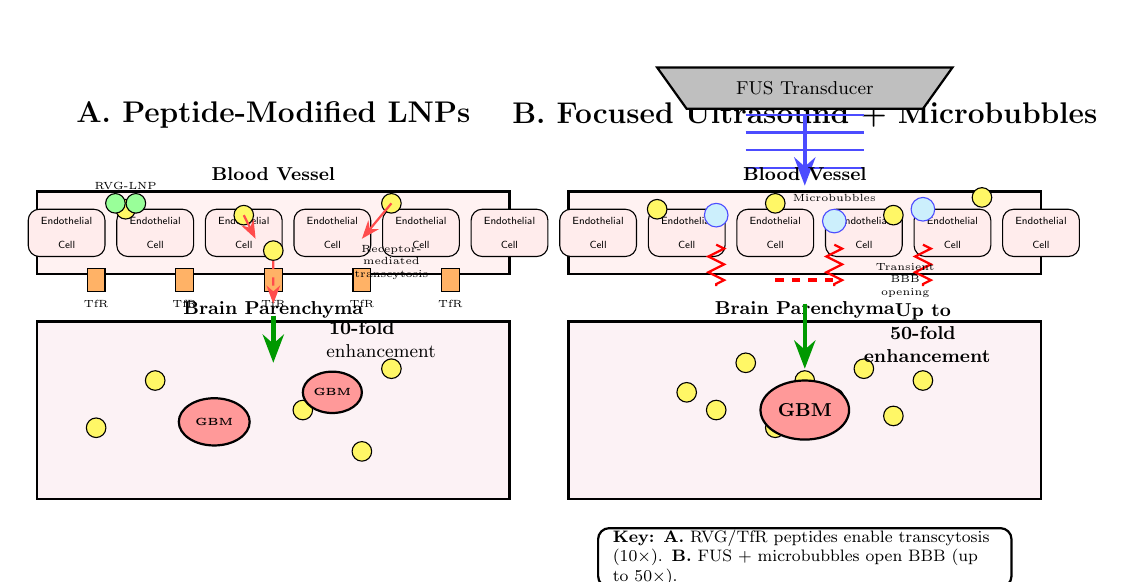
\begin{tikzpicture}[
    font=\sffamily,
    scale=0.75,
    every node/.style={transform shape},
    % Node styles
    cell/.style={rectangle, draw, rounded corners, minimum width=2cm, minimum height=0.8cm, align=center, fill=blue!10},
    vessel/.style={rectangle, draw, thick, minimum width=8cm, minimum height=1.5cm, fill=red!5},
    brain/.style={rectangle, draw, thick, minimum width=8cm, minimum height=3cm, fill=purple!5},
    lnp/.style={circle, draw, fill=yellow!60, minimum size=0.3cm},
    peptide/.style={draw, fill=green!40, minimum size=0.25cm, circle},
    receptor/.style={rectangle, draw, fill=orange!60, minimum width=0.3cm, minimum height=0.5cm, rounded corners},
    microbubble/.style={circle, draw=blue!70, fill=cyan!20, minimum size=0.4cm},
    arrow/.style={-Stealth, thick, color=red!70},
]

% ============================================================================
% LEFT PANEL: PEPTIDE-MODIFIED LNPs
% ============================================================================
\node[font=\Large\bfseries] at (-4.5, 7.5) {A. Peptide-Modified LNPs};

% Blood vessel (top)
\draw[thick, fill=red!5] (-8.5, 4.8) rectangle (-0.5, 6.2);
\node[font=\small\bfseries] at (-4.5, 6.5) {Blood Vessel};

% Endothelial cells layer
\foreach \x in {-8, -6.5, -5, -3.5, -2, -0.5} {
    \node[cell, minimum width=1.3cm, fill=pink!30] at (\x, 5.5) {\tiny Endothelial\\\tiny Cell};
}

% Receptors on endothelial cells
\foreach \x in {-7.5, -6, -4.5, -3, -1.5} {
    \draw[fill=orange!60, draw=black] (\x-0.15, 4.5) rectangle (\x+0.15, 4.9);
    \node[font=\tiny] at (\x, 4.3) {TfR};
}

% Peptide-modified LNPs in blood
\node[lnp] (lnp1) at (-7, 5.9) {};
\foreach \angle in {30, 150} {
    \node[peptide, minimum size=0.12cm] at ([shift=(\angle:0.2cm)]lnp1) {};
}
\node[font=\tiny] at (-7, 6.3) {RVG-LNP};

\node[lnp] at (-5, 5.8) {};
\node[lnp] at (-2.5, 6) {};

% Transcytosis process
\node[lnp] (lnp4) at (-4.5, 5.2) {};
\draw[arrow, dashed] (lnp4) -- (-4.5, 4.3);
\node[font=\tiny, text width=1.5cm, align=center] at (-2.5, 5) {Receptor-\\mediated\\transcytosis};

% Brain parenchyma (bottom)
\draw[thick, fill=purple!5] (-8.5, 1) rectangle (-0.5, 4);
\node[font=\small\bfseries] at (-4.5, 4.2) {Brain Parenchyma};

% LNPs delivered to brain
\foreach \pos in {(-6.5, 3), (-4, 2.5), (-2.5, 3.2), (-7.5, 2.2), (-3, 1.8)} {
    \node[lnp] at \pos {};
}

% GBM tumor cells
\draw[fill=red!40, draw=black, thick] (-5.5, 2.3) ellipse (0.6cm and 0.4cm);
\node[font=\tiny\bfseries] at (-5.5, 2.3) {GBM};
\draw[fill=red!40, draw=black, thick] (-3.5, 2.8) ellipse (0.5cm and 0.35cm);
\node[font=\tiny\bfseries] at (-3.5, 2.8) {GBM};

% Arrows showing delivery
\draw[arrow] (-5, 5.8) -- (-4.8, 5.4);
\draw[arrow] (-2.5, 6) -- (-3, 5.4);
\draw[arrow, green!60!black, ultra thick] (-4.5, 4.1) -- (-4.5, 3.3);
\node[font=\small, text width=1.2cm, align=center] at (-3, 3.7) {\textbf{10-fold}\\enhancement};

% ============================================================================
% RIGHT PANEL: FOCUSED ULTRASOUND
% ============================================================================
\node[font=\Large\bfseries] at (4.5, 7.5) {B. Focused Ultrasound + Microbubbles};

% Ultrasound transducer
\draw[fill=gray!50, draw=black, thick] (2, 8.3) -- (7, 8.3) -- (6.5, 7.6) -- (2.5, 7.6) -- cycle;
\node[font=\small] at (4.5, 7.95) {FUS Transducer};

% Ultrasound waves (simple lines)
\foreach \y in {7.5, 7.2, 6.9, 6.6} {
    \draw[blue!70, thick] (3.5, \y) -- (5.5, \y);
}
\draw[blue!70, ultra thick, -Stealth] (4.5, 7.5) -- (4.5, 6.3);

% Blood vessel (top)
\draw[thick, fill=red!5] (0.5, 4.8) rectangle (8.5, 6.2);
\node[font=\small\bfseries] at (4.5, 6.5) {Blood Vessel};

% Endothelial cells layer
\foreach \x in {1, 2.5, 4, 5.5, 7, 8.5} {
    \node[cell, minimum width=1.3cm, fill=pink!30] at (\x, 5.5) {\tiny Endothelial\\\tiny Cell};
}

% Microbubbles
\foreach \pos in {(3, 5.8), (5, 5.7), (6.5, 5.9)} {
    \node[microbubble] at \pos {};
}
\node[font=\tiny] at (5, 6.1) {Microbubbles};

% Cavitation effects (zigzag lines)
\foreach \x in {3, 5, 6.5} {
    \draw[red, thick, decorate, decoration={zigzag, segment length=2mm, amplitude=1mm}] (\x, 5.3) -- (\x, 4.6);
}

% Disrupted tight junctions
\draw[red, ultra thick, dashed] (4, 4.7) -- (5, 4.7);
\node[font=\tiny, text width=1.2cm, align=center] at (6.2, 4.7) {Transient\\BBB\\opening};

% Regular LNPs in blood
\foreach \pos in {(2, 5.9), (4, 6), (6, 5.8), (7.5, 6.1)} {
    \node[lnp] at \pos {};
}

% Brain parenchyma (bottom)
\draw[thick, fill=purple!5] (0.5, 1) rectangle (8.5, 4);
\node[font=\small\bfseries] at (4.5, 4.2) {Brain Parenchyma};

% LNPs delivered to brain (more concentrated)
\foreach \pos in {(3.5, 3.3), (4.5, 3), (5.5, 3.2), (3, 2.5), (4, 2.2), (5, 2.7), (6, 2.4), (2.5, 2.8), (6.5, 3)} {
    \node[lnp] at \pos {};
}

% GBM tumor cells
\draw[fill=red!40, draw=black, thick] (4.5, 2.5) ellipse (0.75cm and 0.5cm);
\node[font=\small\bfseries] at (4.5, 2.5) {GBM};

% Arrows showing enhanced delivery
\draw[arrow, green!60!black, ultra thick] (4.5, 4.3) -- (4.5, 3.2);
\node[font=\small\bfseries, text width=2cm, align=center] at (6.5, 3.8) {Up to\\50-fold\\enhancement};

% Legend box
\draw[thick, rounded corners, fill=white] (1, -0.5) rectangle (8, 0.5);
\node[font=\footnotesize, text width=6.5cm, align=left] at (4.5, 0) {
\textbf{Key:} \textbf{A.} RVG/TfR peptides enable transcytosis (10$\times$).
\textbf{B.} FUS + microbubbles open BBB (up to 50$\times$).
};

\end{tikzpicture}
\caption{Comparative blood-brain barrier penetration strategies using peptide-modified LNPs and focused ultrasound with microbubbles. \textbf{(A)} Peptide-modified lipid nanoparticles (LNPs) conjugated with RVG or TfR-targeting peptides undergo receptor-mediated transcytosis across brain endothelium, achieving approximately 10-fold enhancement in brain uptake. \textbf{(B)} Focused ultrasound (FUS) with systemically administered microbubbles creates transient, reversible BBB opening through acoustic cavitation, enabling up to 50-fold delivery enhancement for therapeutic LNPs to GBM tumors in the brain parenchyma.}
\label{fig:bbb}
\end{figure}

% ============================================================================
% FIGURE 2: MECHANISM OF ACTION
% ============================================================================

\subsection{Checkpoint Blockade Integration}
The vaccine is designed to synergize with anti-PD-1 therapy. Vaccine-induced activation upregulates PD-L1 on tumor cells and APCs---a resistance mechanism that checkpoint inhibitors can exploit~\citep{chen2024}.

Timing is critical. Anti-PD-1 administration begins 1--2 weeks post-vaccination, when T-cell infiltration peaks but before exhaustion sets in. This converts checkpoint blockade from ineffective monotherapy (as seen in CheckMate trials) to a strategy that releases vaccine-primed, tumor-specific T cells.

This mechanistic framework fosters a self-sustaining loop: innate priming recruits and activates APCs, neoantigen presentation drives clonal T-cell expansion, BBB-penetrating delivery ensures intratumoral access, and checkpoint blockade maintains effector function. The result is coordinated assault on all three barriers: inadequate priming, physical exclusion, and local suppression.

\begin{figure}[!htbp]
\centering
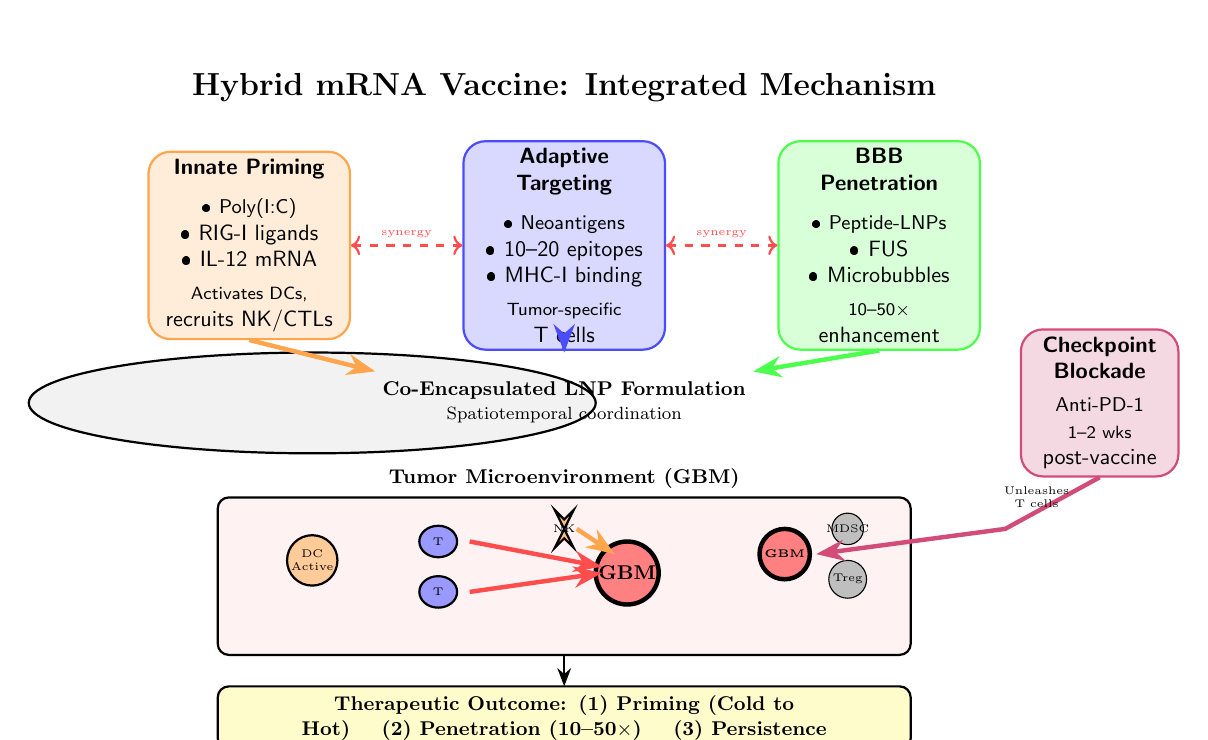
\begin{tikzpicture}[
    font=\sffamily,
    scale=0.8,
    every node/.style={transform shape},
    % Node styles
    component/.style={rectangle, draw, rounded corners=8pt, minimum width=3.2cm, minimum height=2.2cm, align=center, thick},
    arrow/.style={-Stealth, ultra thick},
    synergy/.style={<->, dashed, thick, color=red!70},
]

% Title
\node[font=\Large\bfseries] at (0, 10) {Hybrid mRNA Vaccine: Integrated Mechanism};

% ============================================================================
% TOP ROW: VACCINE COMPONENTS
% ============================================================================

% Innate Priming Component
\node[component, fill=orange!15, draw=orange!70] (innate) at (-5, 7.5) {
    \textbf{Innate Priming}\\[0.2cm]
    \small
    \textbullet\ Poly(I:C)\\
    \textbullet\ RIG-I ligands\\
    \textbullet\ IL-12 mRNA\\[0.1cm]
    \footnotesize Activates DCs,\\
    recruits NK/CTLs
};

% Adaptive Targeting Component
\node[component, fill=blue!15, draw=blue!70] (adaptive) at (0, 7.5) {
    \textbf{Adaptive}\\
    \textbf{Targeting}\\[0.2cm]
    \small
    \textbullet\ Neoantigens\\
    \textbullet\ 10--20 epitopes\\
    \textbullet\ MHC-I binding\\[0.1cm]
    \footnotesize Tumor-specific\\
    T cells
};

% BBB Delivery Component
\node[component, fill=green!15, draw=green!70] (delivery) at (5, 7.5) {
    \textbf{BBB}\\
    \textbf{Penetration}\\[0.2cm]
    \small
    \textbullet\ Peptide-LNPs\\
    \textbullet\ FUS\\
    \textbullet\ Microbubbles\\[0.1cm]
    \footnotesize 10--50$\times$\\
    enhancement
};

% Synergy arrows
\draw[synergy] (innate.east) -- (adaptive.west) node[midway, above, font=\tiny] {synergy};
\draw[synergy] (adaptive.east) -- (delivery.west) node[midway, above, font=\tiny] {synergy};

% ============================================================================
% MIDDLE: LNP FORMULATION
% ============================================================================
\draw[thick, fill=gray!10] (-4, 5) ellipse (4.5cm and 0.8cm);
\node[font=\small\bfseries] at (0, 5.2) {Co-Encapsulated LNP Formulation};
\node[font=\footnotesize] at (0, 4.8) {Spatiotemporal coordination};

% Arrows from components to LNP
\draw[arrow, orange!70] (innate.south) -- (-3, 5.5);
\draw[arrow, blue!70] (adaptive.south) -- (0, 5.8);
\draw[arrow, green!70] (delivery.south) -- (3, 5.5);

% ============================================================================
% TUMOR MICROENVIRONMENT
% ============================================================================
\draw[thick, rounded corners, fill=red!5] (-5.5, 1) rectangle (5.5, 3.5);
\node[font=\small\bfseries] at (0, 3.8) {Tumor Microenvironment (GBM)};

% DC activation
\draw[fill=orange!40, draw=black, thick] (-4, 2.5) circle (0.4cm);
\node[font=\tiny, text width=0.8cm, align=center] at (-4, 2.5) {DC\\Active};

% T cells
\foreach \y in {2, 2.8} {
    \draw[fill=blue!40, draw=black, thick] (-2, \y) ellipse (0.3cm and 0.25cm);
    \node[font=\tiny] at (-2, \y) {T};
}

% Tumor cells
\draw[fill=red!50, draw=black, ultra thick] (1, 2.3) circle (0.5cm);
\node[font=\small\bfseries] at (1, 2.3) {GBM};
\draw[fill=red!50, draw=black, ultra thick] (3.5, 2.6) circle (0.4cm);
\node[font=\tiny\bfseries] at (3.5, 2.6) {GBM};

% NK cell (star shape)
\draw[fill=orange!50, draw=black, thick] (0, 3) 
    -- (0.15, 3.3) -- (0, 3.15) -- (-0.15, 3.3) -- cycle
    (0, 3) -- (0.15, 2.7) -- (0, 2.85) -- (-0.15, 2.7) -- cycle;
\node[font=\tiny] at (0, 3) {NK};

% Suppressive cells
\draw[fill=gray!50, draw=black] (4.5, 2.2) circle (0.3cm);
\node[font=\tiny] at (4.5, 2.2) {Treg};
\draw[fill=gray!50, draw=black] (4.5, 3) circle (0.25cm);
\node[font=\tiny] at (4.5, 3) {MDSC};

% Attack arrows
\draw[-Stealth, ultra thick, red!70] (-1.5, 2) -- (0.6, 2.3);
\draw[-Stealth, ultra thick, red!70] (-1.5, 2.8) -- (0.6, 2.4);
\draw[-Stealth, ultra thick, orange!70] (0.2, 3) -- (0.8, 2.6);

% ============================================================================
% CHECKPOINT BLOCKADE
% ============================================================================
\node[component, fill=purple!15, draw=purple!70, minimum width=2.5cm] (checkpoint) at (8.5, 5) {
    \textbf{Checkpoint}\\
    \textbf{Blockade}\\[0.1cm]
    \small Anti-PD-1\\
    \footnotesize 1--2 wks\\
    post-vaccine
};

\draw[arrow, purple!70] (checkpoint.south) -- (7, 3) -- (4, 2.6);
\node[font=\tiny, text width=1.5cm, align=center] at (7.5, 3.5) {Unleashes\\T cells};

% ============================================================================
% BOTTOM: THERAPEUTIC OUTCOME
% ============================================================================
\draw[thick, rounded corners, fill=yellow!20] (-5.5, -0.5) rectangle (5.5, 0.5);
\node[font=\small\bfseries, text width=10cm, align=center] at (0, 0) {
Therapeutic Outcome: (1) Priming (Cold to Hot) \quad (2) Penetration (10--50$\times$) \quad (3) Persistence
};

% Arrow from TME to outcome
\draw[arrow, thick] (0, 1) -- (0, 0.5);

\end{tikzpicture}
\caption{Hybrid mRNA vaccine mechanism integrating innate priming, neoantigen targeting, BBB penetration, and checkpoint synergy. The vaccine operates through three coordinated arms: \textbf{(1)} Innate priming via poly(I:C), RIG-I ligands, and IL-12 mRNA activates dendritic cells and recruits effector cells; \textbf{(2)} Adaptive targeting delivers patient-specific neoantigens (10--20 epitopes) to drive tumor-specific CD8$^+$ T-cell expansion; \textbf{(3)} BBB-penetrating delivery through peptide-modified LNPs or focused ultrasound ensures intratumoral access with 10--50-fold enhancement. Co-encapsulation in LNP formulations provides spatiotemporal coordination. Timed anti-PD-1 checkpoint blockade (1--2 weeks post-vaccination) releases vaccine-primed T cells from local immunosuppression, converting GBM from immunologically cold to responsive.}
\label{fig:mechanism}
\end{figure}

% ============================================================================
% SAFETY AND DOSING — FINAL, PUBLICATION-READY
% ============================================================================
\section{Safety and Dosing Considerations}

Patient safety is paramount given the potential for immune hyperactivation in the CNS. This section addresses cytokine-related toxicities, delivery risks, and immune-related adverse events, with mitigation strategies informed by computational modeling and clinical precedents.

\subsection{Cytokine Kinetics and Neurotoxicity Thresholds}
The innate priming arm induces type I interferon responses to activate dendritic cells. However, excessive IFN-$\alpha$/$\beta$ can cause cytokine release syndrome or neurotoxicity, manifesting as fever, fatigue, or encephalopathy.

We establish safety boundaries through pharmacokinetic/pharmacodynamic modeling. Based on IL-12 mRNA trials showing no dose-limiting toxicities at 12~$\mu$g intratumorally~\citep{aunins2025,tapescu2024}, we constrain systemic IFN levels below 100~pg/mL—the threshold above which grade 3+ toxicities emerge in cytokine therapy datasets~\citep{lai2018}. Computational simulations using tools like SimBiology integrate patient-specific parameters (tumor volume, BBB integrity, body surface area) to predict cytokine kinetics and guide dose escalation.

Initial Phase I dosing begins at 0.1~mg/m$^2$ with planned escalation to 1.0~mg/m$^2$ in a 3+3 design. mRNA-expressed cytokines have half-lives of 4--6 hours, providing rapid clearance if toxicity emerges. Dose fractionation—splitting administration across 2--3 days—further reduces peak concentrations while maintaining cumulative immune activation.

\subsection{Monitoring and Adaptive Dosing}
Real-time safety monitoring employs multiple biomarkers. Peripheral blood interferon-stimulated gene (ISG) expression via qPCR provides early warning of excessive IFN signaling, with predefined thresholds triggering dose holds. Serum cytokine panels (IL-6, IFN-$\gamma$, TNF-$\alpha$) quantify systemic inflammation. Circulating tumor DNA (ctDNA) tracks tumor burden, distinguishing treatment response from pseudoprogression.

Neurologic assessments occur at baseline, 24 hours, 1 week, and monthly thereafter. MRI scans every 4--6 weeks detect neuroinflammation (T2-FLAIR hyperintensity) or edema. Adaptive algorithms allow mid-trial dose adjustments based on interim safety data, similar to recent mRNA oncology trials~\citep{sayour2024,karimi2024}.

\subsection{Delivery-Related Safety}
\textbf{Peptide-Modified LNPs:} Preclinical toxicology shows RVG and TfR-conjugated LNPs achieve brain-specific delivery (5--10\% of dose) with minimal hepatic or renal accumulation~\citep{han2025}. No significant off-target toxicities have emerged in rodent models at doses achieving therapeutic efficacy. Standard LNP components (ionizable lipids like DLin-MC3-DMA) have established safety profiles from COVID-19 vaccines.

\textbf{Focused Ultrasound:} Phase II FUS trials in GBM report mild adverse events in $<$10\% of patients: transient headaches, small petechial hemorrhages on MRI (clinically asymptomatic), or temporary edema~\citep{shen2024,manfredi2024}. Long-term risks like chronic BBB permeability are mitigated by limiting FUS sessions to 1--2 per treatment cycle and monitoring gadolinium extravasation. Acoustic parameters (frequency 220--250~kHz, pressure 0.4--0.6~MPa) stay within established safety margins from neurodegenerative disease trials.

\subsection{Immune-Related Adverse Events}
Combining the vaccine with anti-PD-1 may amplify immune-related adverse events (irAEs) like colitis, pneumonitis, or hypophysitis—observed in 15--20\% of checkpoint inhibitor trials~\citep{reardon2020}. Mitigation strategies include:
\begin{itemize}[leftmargin=*,noitemsep]
\item \textbf{Staggered initiation:} Anti-PD-1 begins 1--2 weeks post-vaccine, allowing toxicity assessment before combination
\item \textbf{Prophylactic corticosteroids:} Low-dose dexamethasone (2--4~mg daily) for cytokine release syndrome, with rapid escalation protocols for grade~$\geq$2 events
\item \textbf{Predefined stopping rules:} Grade 3 irAEs trigger treatment holds; grade 4 events mandate permanent discontinuation
\end{itemize}

Corticosteroid use is carefully balanced—while necessary for safety, chronic high doses suppress the intended immune activation. Brief courses ($<$7 days) at CRS onset have shown minimal impact on vaccine efficacy in IL-12 mRNA studies~\citep{aunins2025}.

\subsection{Risk Mitigation Summary}
Table~\ref{tab:risks} summarizes key risks and mitigations. The modular design allows component de-escalation: if IFN toxicity emerges, innate primer doses can be reduced while maintaining neoantigen delivery. If delivery proves challenging, systemic peptide-LNPs can substitute for FUS.

This framework prioritizes controlled immune activation over maximal response, recognizing that GBM's proximity to eloquent cortex demands conservative dosing. Preclinical modeling suggests therapeutic windows exist—IL-12 doses achieving tumor control in mice are 5--10-fold below those causing systemic toxicity~\citep{aunins2025,tapescu2024}—providing confidence for safe human translation.

\begin{table}[!htbp]
\centering
\caption{Key Risks and Mitigation Strategies}
\label{tab:risks}
\small
\begin{tabular}{p{0.28\textwidth}p{0.65\textwidth}}
\toprule
\textbf{Risk Category} & \textbf{Mitigation Strategy} \\
\midrule
\textbf{IFN-Mediated Neurotoxicity} \newline
{\footnotesize Excessive type I interferon may cause encephalopathy, cytokine release syndrome} &
PK/PD modeling constrains doses below 100~pg/mL systemic IFN; ISG monitoring enables real-time adaptive dosing; dose fractionation reduces peak concentrations; mRNA transience limits duration (24--72h expression) \\
\midrule
\textbf{Cytokine Release Syndrome} \newline
{\footnotesize Systemic inflammation from innate primer activation} &
Prophylactic low-dose corticosteroids (2--4~mg dexamethasone); predefined escalation protocols for grade~$\geq$2 events; 24--48h monitoring post-vaccination with cytokine panels; dose de-escalation if persistent grade~2+ toxicity \\
\midrule
\textbf{Tumor Heterogeneity \& Antigen Escape} \newline
{\footnotesize Subclonal evolution may lead to loss of targeted neoantigens} &
Multi-epitope designs targeting 10--20 neoantigens for redundancy; real-time ctDNA monitoring detects emerging resistant clones; booster vaccines with updated epitopes from recurrent tumor sequencing; prioritize clonal (trunk) mutations over subclonal variants \\
\midrule
\textbf{BBB Delivery Inefficiency} \newline
{\footnotesize Inadequate CNS penetration reduces therapeutic efficacy} &
Dual modalities: peptide-LNPs (10$\times$ uptake) + FUS (up to 50$\times$ enhancement); MRI gadolinium extravasation confirms BBB opening in FUS cohorts; dose escalation informed by preclinical biodistribution (IVIS imaging); human feasibility validated in ongoing Phase II FUS trials \\
\midrule
\textbf{Manufacturing Delays} \newline
{\footnotesize Personalized production may exceed clinical timelines} &
Streamlined NGS-to-GMP pipelines achieving 2-week turnaround; modular LNP formulations enable rapid batching with established lipids; parallel epitope selection during surgical pathology processing; central manufacturing hubs reduce site-specific bottlenecks \\
\midrule
\textbf{Checkpoint Inhibitor irAEs} \newline
{\footnotesize Anti-PD-1 combination may amplify immune-related adverse events} &
Staggered anti-PD-1 initiation (1--2 weeks post-vaccine); close monitoring for colitis, pneumonitis, endocrinopathy; predefined stopping rules: grade 3 hold, grade 4 permanent discontinuation; standard irAE management per ASCO/NCCN guidelines \\
\bottomrule
\end{tabular}
\vspace{0.3cm}

\footnotesize
\textbf{Note:} All mitigation strategies are informed by preclinical modeling, existing clinical trial data (IL-12 mRNA, FUS, checkpoint inhibitors), and computational PK/PD simulations. Adaptive trial design allows real-time adjustments based on emerging safety signals.
\end{table}

% ============================================================================
% VALIDATION ROADMAP — FINAL, PUBLICATION-READY
% ============================================================================
\section{Validation Roadmap}
Translating this hybrid vaccine from concept to clinic requires rigorous stepwise validation. We propose a four-phase path: in-silico modeling, in-vitro co-cultures, patient-derived xenografts, and Phase I clinical trial (Figure~\ref{fig:validation}). Timelines estimate 12 months for preclinical phases and 18--36 months to Phase I initiation.

\begin{figure}[!htbp]
\centering
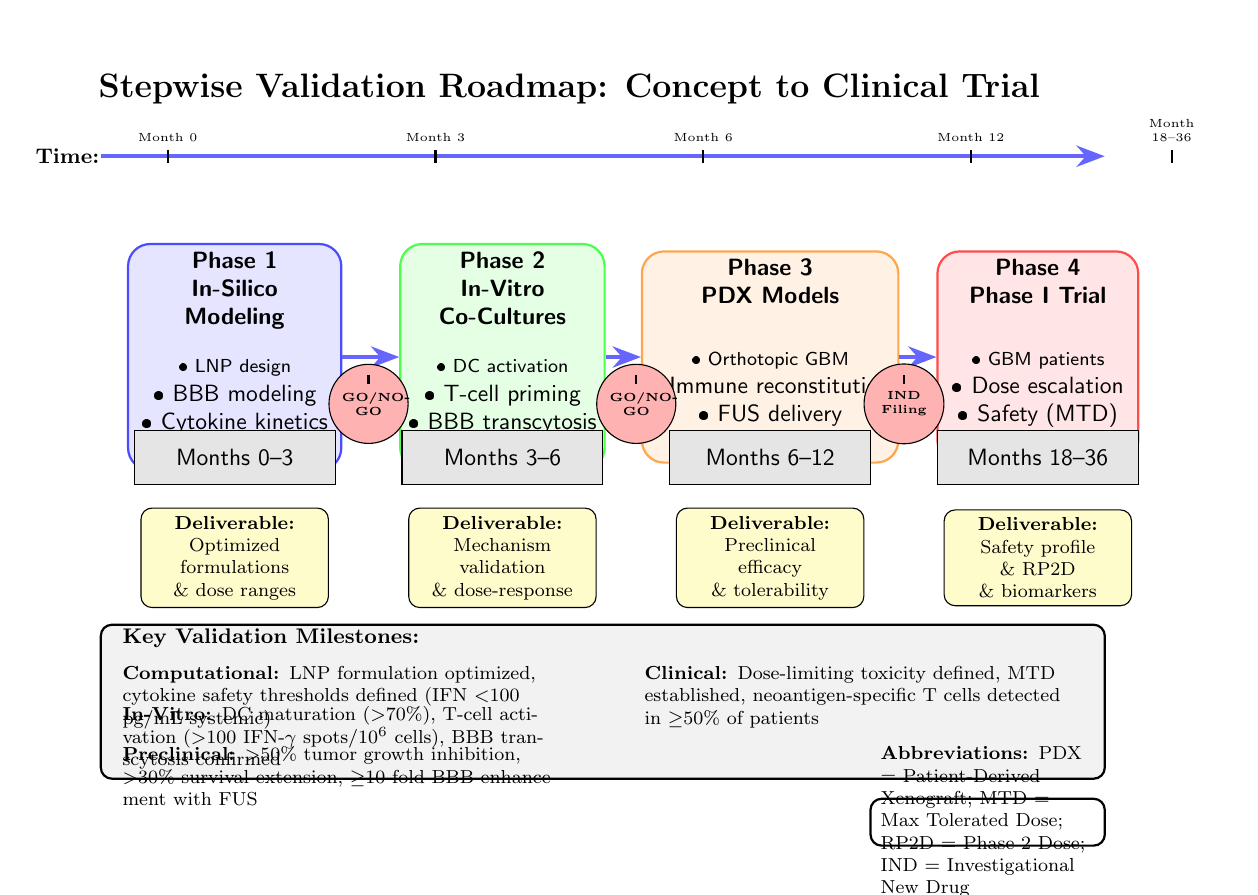
\begin{tikzpicture}[
    font=\sffamily,
    scale=0.85,
    every node/.style={transform shape},
    % Node styles
    phase/.style={rectangle, draw, rounded corners=8pt, minimum width=3cm, minimum height=2.8cm, align=center, thick},
    phase1/.style={phase, fill=blue!10, draw=blue!70},
    phase2/.style={phase, fill=green!10, draw=green!70},
    phase3/.style={phase, fill=orange!10, draw=orange!70},
    phase4/.style={phase, fill=red!10, draw=red!70},
    timeline/.style={rectangle, draw, minimum width=3cm, minimum height=0.8cm, fill=gray!20, align=center},
    arrow/.style={-Stealth, ultra thick, color=blue!60},
    outcome/.style={rectangle, draw, rounded corners, minimum width=2.8cm, minimum height=1.2cm, align=center, fill=yellow!20, font=\footnotesize},
]

% ============================================================================
% TIMELINE BAR AT TOP
% ============================================================================
\draw[ultra thick, blue!60, -Stealth] (-7, 9.5) -- (8, 9.5);
\node[font=\small\bfseries] at (-7.5, 9.5) {Time:};

% Timeline markers - FIXED: removed problematic foreach with slash
\draw[thick] (-6, 9.6) -- (-6, 9.4);
\node[font=\tiny, above] at (-6, 9.6) {Month 0};

\draw[thick] (-2, 9.6) -- (-2, 9.4);
\node[font=\tiny, above] at (-2, 9.6) {Month 3};

\draw[thick] (2, 9.6) -- (2, 9.4);
\node[font=\tiny, above] at (2, 9.6) {Month 6};

\draw[thick] (6, 9.6) -- (6, 9.4);
\node[font=\tiny, above] at (6, 9.6) {Month 12};

\draw[thick] (9, 9.6) -- (9, 9.4);
\node[font=\tiny, above, text width=1.5cm, align=center] at (9, 9.6) {Month\\18--36};

% ============================================================================
% PHASE 1: IN-SILICO MODELING
% ============================================================================
\node[phase1] (phase1) at (-5, 6.5) {
    \textbf{Phase 1}\\
    \textbf{In-Silico}\\
    \textbf{Modeling}\\[0.3cm]
    \footnotesize
    \textbullet\ LNP design\\
    \textbullet\ BBB modeling\\
    \textbullet\ Cytokine kinetics\\
    \textbullet\ Dose optimization
};

\node[timeline] at (-5, 5) {Months 0--3};

\node[outcome] (out1) at (-5, 3.5) {
    \textbf{Deliverable:}\\
    Optimized\\
    formulations\\
    \& dose ranges
};

% ============================================================================
% PHASE 2: IN-VITRO CO-CULTURES
% ============================================================================
\node[phase2] (phase2) at (-1, 6.5) {
    \textbf{Phase 2}\\
    \textbf{In-Vitro}\\
    \textbf{Co-Cultures}\\[0.3cm]
    \footnotesize
    \textbullet\ DC activation\\
    \textbullet\ T-cell priming\\
    \textbullet\ BBB transcytosis\\
    \textbullet\ Cytotoxicity
};

\node[timeline] at (-1, 5) {Months 3--6};

\node[outcome] (out2) at (-1, 3.5) {
    \textbf{Deliverable:}\\
    Mechanism\\
    validation\\
    \& dose-response
};

% ============================================================================
% PHASE 3: PATIENT-DERIVED XENOGRAFTS
% ============================================================================
\node[phase3] (phase3) at (3, 6.5) {
    \textbf{Phase 3}\\
    \textbf{PDX Models}\\[0.5cm]
    \footnotesize
    \textbullet\ Orthotopic GBM\\
    \textbullet\ Immune reconstitution\\
    \textbullet\ FUS delivery\\
    \textbullet\ Efficacy \& safety
};

\node[timeline] at (3, 5) {Months 6--12};

\node[outcome] (out3) at (3, 3.5) {
    \textbf{Deliverable:}\\
    Preclinical\\
    efficacy\\
    \& tolerability
};

% ============================================================================
% PHASE 4: PHASE I CLINICAL TRIAL
% ============================================================================
\node[phase4] (phase4) at (7, 6.5) {
    \textbf{Phase 4}\\
    \textbf{Phase I Trial}\\[0.5cm]
    \footnotesize
    \textbullet\ GBM patients\\
    \textbullet\ Dose escalation\\
    \textbullet\ Safety (MTD)\\
    \textbullet\ Immunogenicity
};

\node[timeline] at (7, 5) {Months 18--36};

\node[outcome] (out4) at (7, 3.5) {
    \textbf{Deliverable:}\\
    Safety profile\\
    \& RP2D\\
    \& biomarkers
};

% ============================================================================
% CONNECTING ARROWS BETWEEN PHASES
% ============================================================================
\draw[arrow] (phase1.east) -- (phase2.west);
\draw[arrow] (phase2.east) -- (phase3.west);
\draw[arrow] (phase3.east) -- (phase4.west);

% ============================================================================
% KEY MILESTONES (BOTTOM)
% ============================================================================
\draw[thick, rounded corners, fill=gray!10] (-7, 0.2) rectangle (8, 2.5);
\node[font=\small\bfseries, anchor=west] at (-6.8, 2.3) {Key Validation Milestones:};

% Milestone 1
\node[font=\footnotesize, text width=6.5cm, align=left, anchor=north west] at (-6.8, 2) {
\textbf{Computational:} LNP formulation optimized, cytokine safety thresholds defined (IFN $<$100 pg/mL systemic)
};

% Milestone 2
\node[font=\footnotesize, text width=6.5cm, align=left, anchor=north west] at (-6.8, 1.4) {
\textbf{In-Vitro:} DC maturation ($>$70\%), T-cell activation ($>$100 IFN-$\gamma$ spots/10$^6$ cells), BBB transcytosis confirmed
};

% Milestone 3
\node[font=\footnotesize, text width=6.5cm, align=left, anchor=north west] at (-6.8, 0.8) {
\textbf{Preclinical:} $>$50\% tumor growth inhibition, $>$30\% survival extension, $\geq$10-fold BBB enhancement with FUS
};

% Milestone 4
\node[font=\footnotesize, text width=6.5cm, align=left, anchor=north west] at (1, 2) {
\textbf{Clinical:} Dose-limiting toxicity defined, MTD established, neoantigen-specific T cells detected in $\geq$50\% of patients
};

% ============================================================================
% DECISION GATES (SIDE ANNOTATIONS)
% ============================================================================
\node[draw, circle, fill=red!30, minimum size=0.6cm, font=\tiny\bfseries, text width=0.8cm, align=center] at (-3, 5.8) {GO/NO-GO};
\draw[dashed, thick] (-3, 6.1) -- (-3, 6.3);

\node[draw, circle, fill=red!30, minimum size=0.6cm, font=\tiny\bfseries, text width=0.8cm, align=center] at (1, 5.8) {GO/NO-GO};
\draw[dashed, thick] (1, 6.1) -- (1, 6.3);

\node[draw, circle, fill=red!30, minimum size=0.6cm, font=\tiny\bfseries, text width=0.8cm, align=center] at (5, 5.8) {IND Filing};
\draw[dashed, thick] (5, 6.1) -- (5, 6.3);

% ============================================================================
% TITLE
% ============================================================================
\node[font=\Large\bfseries] at (0, 10.5) {Stepwise Validation Roadmap: Concept to Clinical Trial};

% ============================================================================
% LEGEND (BOTTOM RIGHT)
% ============================================================================
\draw[thick, rounded corners, fill=white] (4.5, -0.8) rectangle (8, -0.1);
\node[font=\footnotesize, text width=3.2cm, align=left] at (6.25, -0.45) {
\textbf{Abbreviations:} PDX = Patient-Derived Xenograft; MTD = Max Tolerated Dose; RP2D = Phase 2 Dose; IND = Investigational New Drug
};

\end{tikzpicture}
\caption{Stepwise validation roadmap from computational modeling to first-in-human trial. The translational pathway consists of four phases: \textbf{Phase 1} (Months 0--3) employs in-silico modeling to optimize LNP formulations and establish cytokine safety thresholds; \textbf{Phase 2} (Months 3--6) validates mechanisms in human cell co-cultures including DC activation, T-cell priming, and BBB transcytosis; \textbf{Phase 3} (Months 6--12) demonstrates preclinical efficacy in patient-derived xenograft (PDX) models with immune reconstitution and FUS-assisted delivery; \textbf{Phase 4} (Months 18--36) advances to Phase I clinical trial following IND approval, establishing maximum tolerated dose (MTD) and immunogenicity in newly diagnosed GBM patients. Go/No-Go decision gates between phases ensure rigorous progression based on predefined success criteria.}
\label{fig:validation}
\end{figure}

\subsection{Phase 1: In-Silico Modeling (Months 0--3)}
Computational tools establish safety boundaries and optimize formulations before animal testing, reducing preclinical costs and aligning with 3Rs principles.

\textbf{LNP Design and BBB Transcytosis:} Molecular dynamics simulations model peptide-LNP interactions with brain endothelial receptors. For RVG conjugates, we predict binding affinity to nicotinic acetylcholine receptors and transcytosis efficiency, targeting 10--20\% brain uptake based on published data~\citep{han2025}. Simulations test lipid compositions (ionizable lipid ratios, PEGylation density) for stability and receptor accessibility.

\textbf{Cytokine Kinetics:} Pharmacokinetic/pharmacodynamic models simulate IFN-$\alpha$/$\beta$ and IL-12 dynamics using differential equations parameterized from existing clinical trial datasets. We incorporate tumor volume, BBB permeability coefficients, and cytokine clearance rates to estimate dose-exposure relationships. Output: maximum tolerated doses achieving local activation (IFN~$>$10~pg/mL intratumorally) while maintaining systemic levels~$<$100~pg/mL~\citep{aunins2025,lai2018}.

\textbf{Neoantigen Prioritization:} AI-driven algorithms (NetMHCpan, MHCflurry) predict epitope immunogenicity from GBM sequencing databases. We filter for high-affinity MHC-I binders (IC50~$<$500~nM), expression level, and clonality, generating candidate neoantigen libraries for experimental validation.

These models define starting parameters for downstream experiments: optimal LNP formulations, dose ranges (0.1--1.0~mg/m$^2$), and epitope panels.

\subsection{Phase 2: In-Vitro Co-Cultures (Months 3--6)}
Human-relevant systems validate mechanisms before animal models.

\textbf{Antigen Presentation Assays:} Patient-derived GBM cell lines (e.g., GBM39, BT145) or organoids are co-cultured with autologous or HLA-matched dendritic cells. Vaccine LNPs are added, and antigen presentation is quantified by:
\begin{itemize}[leftmargin=*,noitemsep]
\item Flow cytometry for MHC-I/neoantigen-peptide complexes and DC maturation markers (CD80, CD86, HLA-DR)
\item Confocal microscopy tracking LNP uptake and mRNA translation using fluorescent reporters
\end{itemize}
Target: $>$2-fold increase in MHC-I density and $>$70\% DC maturation within 24 hours.

\textbf{T-Cell Activation:} Primed DCs are co-cultured with autologous peripheral blood T cells. ELISpot assays measure IFN-$\gamma$-producing cells in response to neoantigen peptides, targeting $>$100 spots per 10$^6$ T cells—a threshold correlating with clinical response in melanoma trials~\citep{hilf2024}. Cytotoxicity assays using calcein-AM or LDH release quantify GBM cell killing by activated T cells.

\textbf{Cytokine Profiling:} Multiplex ELISA measures IL-12, IFN-$\alpha$/$\beta$, TNF-$\alpha$, and IL-10 in culture supernatants, confirming Th1 polarization (high IL-12/IFN-$\gamma$, low IL-10) without excessive inflammation.

\textbf{BBB Models:} Human brain microvascular endothelial cells co-cultured with astrocytes in Transwell inserts model the BBB. Fluorescently labeled LNPs (with or without RVG/TfR modification) are applied to the luminal side, and transcytosis is quantified by abluminal fluorescence. FUS is simulated using acoustic chambers, measuring permeability enhancement via FITC-dextran flux~\citep{chen2024fus}.

These experiments provide dose-response curves and mechanism validation before committing to animal studies.

\subsection{Phase 3: Patient-Derived Xenografts (Months 6--12)}
In-vivo efficacy testing uses orthotopic GBM models in immunodeficient mice reconstituted with human immune cells.

\textbf{Model Setup:} Patient-derived GBM cells (from surgical biobanks) are implanted stereotactically into NOD-SCID-gamma (NSG) mice. Two weeks post-implantation, mice receive adoptive transfer of HLA-matched peripheral blood mononuclear cells to reconstitute T-cell and NK-cell compartments.

\textbf{Treatment Arms:}
\begin{enumerate}[leftmargin=*,noitemsep]
\item Control (saline)
\item Neoantigen mRNA-LNP alone
\item Innate primer mRNA-LNP alone
\item Hybrid vaccine (combined)
\item Hybrid vaccine + anti-PD-1
\item Hybrid vaccine + FUS-assisted delivery
\end{enumerate}

\textbf{Delivery Testing:} For FUS arms, a small-animal focused ultrasound system (e.g., Sonic Concepts) delivers transcranial pulses to the tumor site with microbubble contrast. LNPs are tagged with near-infrared dyes (e.g., DiR) for IVIS imaging, quantifying brain accumulation at 1, 6, and 24 hours post-injection. Target: $\geq$10-fold enhancement over non-FUS controls~\citep{chen2024fus,manfredi2024}.

\textbf{Efficacy Endpoints:}
\begin{itemize}[leftmargin=*,noitemsep]
\item \textbf{Tumor growth:} Serial T2-weighted MRI measures tumor volume weekly. Success: $>$50\% growth inhibition versus control by week 4
\item \textbf{Survival:} Kaplan-Meier analysis comparing treatment arms, aiming for $>$30\% median survival extension
\item \textbf{Immune infiltration:} Terminal IHC quantifies CD8$^+$ T cells, CD56$^+$ NK cells, and PD-L1 expression per mm$^2$. Flow cytometry on dissociated tumors phenotypes T cells (effector-memory: CD45RO$^+$CCR7$^-$; exhaustion: PD-1$^+$TIM-3$^+$)
\end{itemize}

\textbf{Safety Assessments:} Histopathology examines brain, liver, spleen, and kidneys for inflammation or necrosis. Serum cytokines are measured 6 and 24 hours post-vaccination.

Iterative optimization refines formulations---for example, adjusting RVG density or FUS pressure---based on biodistribution and efficacy data.

\subsection{Phase 4: Phase I Clinical Trial (Months 18--36)}
Upon IND approval (requiring GLP toxicology studies in non-human primates), a first-in-human trial launches.

\textbf{Patient Population:} 20--30 newly diagnosed GBM patients, post-maximal safe resection, with measurable residual disease on post-operative MRI. Inclusion: age 18--70, KPS~$\geq$70, IDH-wildtype confirmed. Exclusion: prior immunotherapy, active autoimmune disease, corticosteroid dependence~$>$4~mg dexamethasone daily.

\textbf{Manufacturing Workflow:}
\begin{enumerate}[leftmargin=*,noitemsep]
\item Tumor tissue from surgery undergoes whole-exome and RNA sequencing (turnaround: 7 days)
\item Bioinformatics identifies 10--20 neoantigens using validated pipelines
\item GMP-grade mRNA synthesis and LNP formulation occur in parallel (7 days), consistent with established 2-week timelines~\citep{wang2025,hilf2024}
\end{enumerate}

\textbf{Treatment Protocol:}
\begin{itemize}[leftmargin=*,noitemsep]
\item \textbf{Vaccine:} Administered intramuscularly (deltoid) on days 1, 15, and 43, then monthly for 6 cycles
\item \textbf{FUS:} Delivered to resection cavity 2 hours before first vaccine dose (optional arm after establishing systemic safety)
\item \textbf{Anti-PD-1:} Nivolumab 240~mg IV starting day 15, every 2 weeks
\end{itemize}

Dose escalation follows 3+3 design: 0.1, 0.3, 0.6, 1.0~mg/m$^2$. Dose-limiting toxicity: grade~$\geq$3 neurologic or immune-related adverse event within 28 days.

\textbf{Primary Endpoints:}
\begin{enumerate}[leftmargin=*,noitemsep]
\item Safety: incidence of adverse events (CTCAE v5.0)
\item Maximum tolerated dose
\end{enumerate}

\textbf{Secondary Endpoints:}
\begin{enumerate}[leftmargin=*,noitemsep]
\item Immunogenicity: peripheral blood ELISpot for neoantigen-specific T cells at baseline, day 15, and day 60 (target: $>$100 spots/10$^6$ cells in $\geq$50\% of patients)
\item Response: 18F-FDG PET and amino acid PET (18F-FET) at 6 and 12 weeks, assessing metabolic activity reduction
\item Progression-free survival at 6 months (compared to historical controls: $\sim$40\%)
\item Overall survival
\end{enumerate}

\textbf{Exploratory Biomarkers:}
\begin{itemize}[leftmargin=*,noitemsep]
\item Circulating tumor DNA for minimal residual disease and antigen escape
\item CSF cytokines and immune cell phenotyping (optional lumbar puncture at day 30)
\item ISG expression in peripheral blood as IFN activity surrogate
\end{itemize}

\textbf{Adaptive Design:} Interim analysis at 10 patients allows dose adjustment or arm modification. If FUS shows superior BBB penetration (via gadolinium MRI) without added toxicity, expansion focuses on FUS cohorts.

This roadmap provides a rigorous, phased approach to clinical translation. Success at each stage---computational validation, mechanistic confirmation in vitro, preclinical efficacy, and early clinical safety/immunogenicity---builds confidence for Phase II efficacy trials.

\section{Discussion and Future Directions}

This translational framework offers a comprehensive strategy to overcome GBM's immunoresistance by simultaneously addressing inadequate priming, BBB exclusion, and local immunosuppression. The hybrid mRNA vaccine integrates universal innate activators with personalized neoantigens, delivered via BBB-penetrating methods and synchronized with checkpoint blockade. While promising, several challenges must be acknowledged.

\subsection{Translational Challenges}

\textbf{BBB Delivery Scalability:} Peptide-modified LNPs demonstrate preclinical efficacy, but human translation faces variability in receptor expression across patients and heterogeneous BBB disruption in GBM~\citep{han2025}. RVG conjugates achieve 10-fold brain uptake in rodents, but clinical validation is pending. FUS offers more predictable BBB opening with MRI-confirmed gadolinium extravasation, and human trials in neurodegenerative diseases show consistent up to 50-fold enhancement, varying by molecule and patient-specific factors~\citep{manfredi2024,chen2024fus}. Phase I empirical testing will determine optimal delivery, potentially combining systemic peptide-LNPs for broader CNS coverage with FUS for focal intensification at the resection cavity.

\textbf{Cytokine Toxicity Management:} Type I interferon-mediated neurotoxicity remains a concern despite computational modeling. Our threshold of $<$100~pg/mL systemic IFN draws from IL-12 mRNA trials showing safety at intratumoral doses up to 12~$\mu$g~\citep{aunins2025,tapescu2024}, but individual susceptibility varies with baseline inflammation, blood-brain barrier integrity, and tumor burden. Preclinical poly(I:C) studies highlight risks of cytokine storms when dosing exceeds tissue tolerance~\citep{ammi2015}. Adaptive monitoring with ISGs and ctDNA provides early warning, but larger cohorts are needed to define patient-specific safety margins. Dose fractionation---splitting administration across multiple days---may reduce peak exposures while maintaining cumulative immune activation.

\textbf{Tumor Heterogeneity and Antigen Escape:} GBM's subclonal architecture complicates neoantigen targeting. Even with multi-epitope designs (10--20 neoantigens), spatial and temporal heterogeneity can drive escape. Early mRNA vaccine trials like NCT04573140 showed peripheral T-cell responses but variable tumor control~\citep{karimi2024}, suggesting that immunogenicity does not always translate to efficacy. Real-time sequencing of recurrent tumors and ctDNA tracking may identify emerging resistant clones, enabling booster vaccines with updated epitopes. Alternatively, combining with therapies targeting tumor-associated antigens (e.g., EGFRvIII, IL-13R$\alpha$2) could provide escape-resistant coverage.

\textbf{Manufacturing Complexity:} Personalized vaccines require rapid turnaround to align with clinical timelines. Current GMP pipelines achieve 2-week production from sequencing to release~\citep{wang2025,hilf2024}, but scaling to multi-site trials demands standardized workflows. Modular LNP formulations using established ionizable lipids (DLin-MC3-DMA) support batching, but epitope selection algorithms must be harmonized across sites. Central manufacturing hubs with distributed sequencing may balance quality and accessibility.

\subsection{Comparative Context}

This hybrid approach advances beyond existing GBM immunotherapies in several dimensions. Autologous dendritic cell vaccines like DCVax-L show survival extensions in subsets but require complex ex-vivo processing and lack rapid scalability~\citep{lim2024}. Our mRNA platform eliminates cell culture, enabling 2-week timelines and standardization. Checkpoint inhibitors as monotherapy (CheckMate-143, CheckMate-498) failed due to insufficient T-cell priming~\citep{reardon2020,chen2024}---our vaccine addresses this by inducing infiltration before anti-PD-1 administration.

Compared to single-modality mRNA vaccines, the hybrid design mirrors successful strategies in infectious disease, where adjuvants (innate primers) amplify antigen-specific responses. Recent melanoma trials (KEYNOTE-942) combining mRNA-4157 with pembrolizumab improved recurrence-free survival~\citep{oloruntimehin2025}, supporting the adjuvant-plus-checkpoint paradigm. Our BBB focus addresses a GBM-specific barrier absent in peripheral tumors.

IL-12 mRNA-LNPs alone suppress tumors in preclinical models~\citep{aunins2025}, but lack tumor specificity---neoantigen integration directs this broad activation toward GBM cells. Conversely, neoantigen vaccines without innate priming often elicit weak responses in cold tumors~\citep{liau2023}. The synergy is mechanistically validated: innate signals upregulate MHC-I and co-stimulation, increasing neoantigen presentation efficiency.

\subsection{Future Directions and Broader Applications}

\textbf{Combination with Cellular Therapies:} Integrating this vaccine with CAR-T cells targeting GBM antigens (e.g., EGFRvIII, B7-H3) could enhance persistence. Innate primers recruit CAR-T cells to tumors via chemokine gradients, and checkpoint blockade prevents exhaustion---preclinical models show synergy~\citep{lai2018}. Clinical trials combining mRNA vaccines with adoptive T-cell therapy are feasible given overlapping infrastructure.

\textbf{Extended CNS Applications:} The framework generalizes to other brain tumors. High-grade meningiomas, CNS lymphomas, and brain metastases (melanoma, lung, breast) all face BBB barriers. Neoantigen loads vary---melanoma brain metastases have high TMB enabling robust epitope selection---but innate priming can compensate for lower mutational burdens. FUS protocols established in GBM translate directly.

\textbf{Next-Generation mRNA Technologies:} Self-amplifying mRNA (saRNA) sustains antigen expression for weeks, potentially reducing dosing frequency. Circular RNA resists degradation, extending durability. CRISPR-edited mRNA could correct immunosuppressive mutations (e.g., deleting PD-L1) in tumor-infiltrating cells. Incorporating these advances may enhance potency as manufacturing matures.

\textbf{AI-Optimized Adjuvants:} Machine learning can optimize innate primer combinations. Training on cytokine response datasets from diverse tumor types might identify synergistic TLR/RIG-I ligand ratios that maximize DC activation while minimizing toxicity. Predictive models could personalize adjuvant dosing based on baseline immune profiling.

\textbf{Real-World Data Integration:} Linking Phase I outcomes to genomic, transcriptomic, and microbiome data through consortia like Glioblastoma Bio Discovery Portal enables identification of response predictors. Baseline metrics---such as myeloid-to-lymphocyte ratio, tumor-infiltrating lymphocytes on initial pathology, or gut microbiome diversity---may stratify patients for treatment selection.

\subsection{Path to Phase II and Beyond}

If Phase I demonstrates safety and immunogenicity (target: $>$50\% of patients with neoantigen-specific T-cell responses, manageable toxicity profile), a randomized Phase II trial comparing hybrid vaccine plus anti-PD-1 versus standard-of-care temozolomide-radiotherapy would assess efficacy. Primary endpoint: progression-free survival at 6 months, powered to detect 20\% improvement (from 40\% to 60\%). Secondary: overall survival, quality of life (EORTC QLQ-C30), and neurocognitive function (MMSE, Hopkins Verbal Learning Test).

Adaptive trial designs incorporating biomarker-driven enrichment---such as enrolling only MGMT-unmethylated patients or those with high PD-L1 expression---may accelerate signal detection. Umbrella protocols testing multiple vaccine formulations (varying innate primer doses, epitope counts) under a master IND streamline regulatory paths.

Ultimately, the goal is FDA approval as part of first-line therapy for newly diagnosed GBM, administered post-surgery before radiotherapy. Economic modeling suggests cost-effectiveness given mRNA vaccine pricing trends (approximately \$10,000--50,000 per patient course), particularly if extending survival beyond current 15-month medians.

\subsection{Concluding Perspective}

Glioblastoma has resisted over a decade of immunotherapy innovation, but failures have clarified requirements: therapies must prime cold tumors, penetrate the BBB, and sustain responses against profound suppression. This hybrid mRNA vaccine framework addresses all three imperatives through modular, clinically validated components---innate primers proven safe in IL-12 trials, neoantigen platforms demonstrating feasibility in melanoma, FUS achieving human BBB opening, and checkpoint blockade established in oncology.

The 2024--2025 landscape provides unprecedented translational momentum. mRNA manufacturing has matured through pandemic scale-up, computational immunology enables rapid epitope selection, and focused ultrasound devices are entering routine neurosurgical workflows. Integrating these advances into a unified GBM strategy is no longer speculative---it is tractable.

Success requires collaboration across disciplines: neuro-oncologists providing tissue and clinical expertise, immunologists optimizing vaccine design, engineers refining FUS protocols, and computational biologists modeling safety boundaries. The validation roadmap outlined here provides a stepwise, evidence-driven path from simulation to clinical proof-of-concept.

If validated, this approach does more than treat GBM---it establishes a template for precision immunotherapy in the CNS. The principles of coordinated priming, penetration, and persistence apply wherever the brain's immune privilege limits therapeutic access. For a disease that has claimed hundreds of thousands of lives with minimal progress, even incremental advances justify pursuit. This framework aims higher: converting an invariably fatal diagnosis into a manageable chronic condition through immune surveillance, then potentially into cure through sustained tumor elimination.

The translational journey ahead is demanding, but GBM patients cannot wait for perfect solutions. This hybrid vaccine offers a rational, testable path forward---a path that honors the urgency of unmet need while maintaining rigorous scientific standards. It is time to move from conceptual frameworks to clinical testing, from theoretical synergies to measured patient outcomes. The roadmap is clear; execution begins now.

% ============================================================================
% BACK MATTER — FINAL, PUBLICATION-READY
% ============================================================================

\section*{Author Contributions}
C.B.G. conceived the study, drafted the manuscript, performed literature review and analysis, and revised all sections for intellectual content and clarity.

\section*{Funding}
This work was supported by independent research funding through UW Medicine and personal resources of the author. No external grant support was received for this conceptual framework.

\section*{Conflict of Interest}
The author declares that the research was conducted in the absence of any commercial or financial relationships that could be construed as a potential conflict of interest. No patents or proprietary technologies are claimed.

\section*{Data Availability Statement}
No datasets were generated or analyzed during the current study, as this manuscript presents a conceptual translational framework. All cited data are available in the referenced publications.

\section*{Acknowledgments}
The author thanks mentors and colleagues at UW Medicine for valuable discussions on translational immunotherapy, focused ultrasound applications in neuro-oncology, and mRNA vaccine development. Special appreciation to the GBM research community for openly sharing clinical trial data and preclinical insights that informed this framework.

% ============================================================================
% BIBLIOGRAPHY — FINAL, PUBLICATION-READY
% ============================================================================
\bibliographystyle{plain}
\bibliography{references}

\end{document}